% Generated by Sphinx.
\def\sphinxdocclass{report}
\documentclass[a4paper,oneside,10pt,russian]{sphinxmanual}
\usepackage[utf8]{inputenc}
\DeclareUnicodeCharacter{00A0}{\nobreakspace}
\usepackage{cmap}
\usepackage[T1]{fontenc}
\usepackage{babel}

\usepackage[Sonny]{fncychap}
\usepackage{longtable}
\usepackage{sphinx}
\usepackage{multirow}

\addto\captionsrussian{\renewcommand{\figurename}{Fig. }}
\addto\captionsrussian{\renewcommand{\figurename}{Рис. }}
\addto\captionsrussian{\renewcommand{\tablename}{Table }}
\floatname{literal-block}{Listing }



\title{Набор инструментов мастера-сюжетника НИМС. Документация}
\date{25.11.2015}
\release{0.4.1}
\author{Тимофей NtsDK Речкалов\and Мария Матильда Сидехменова}
\newcommand{\sphinxlogo}{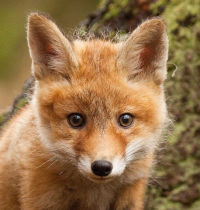
\includegraphics{logo.png}\par}
\renewcommand{\releasename}{Выпуск}
\makeindex

\makeatletter
\def\PYG@reset{\let\PYG@it=\relax \let\PYG@bf=\relax%
    \let\PYG@ul=\relax \let\PYG@tc=\relax%
    \let\PYG@bc=\relax \let\PYG@ff=\relax}
\def\PYG@tok#1{\csname PYG@tok@#1\endcsname}
\def\PYG@toks#1+{\ifx\relax#1\empty\else%
    \PYG@tok{#1}\expandafter\PYG@toks\fi}
\def\PYG@do#1{\PYG@bc{\PYG@tc{\PYG@ul{%
    \PYG@it{\PYG@bf{\PYG@ff{#1}}}}}}}
\def\PYG#1#2{\PYG@reset\PYG@toks#1+\relax+\PYG@do{#2}}

\expandafter\def\csname PYG@tok@gd\endcsname{\def\PYG@tc##1{\textcolor[rgb]{0.63,0.00,0.00}{##1}}}
\expandafter\def\csname PYG@tok@gu\endcsname{\let\PYG@bf=\textbf\def\PYG@tc##1{\textcolor[rgb]{0.50,0.00,0.50}{##1}}}
\expandafter\def\csname PYG@tok@gt\endcsname{\def\PYG@tc##1{\textcolor[rgb]{0.00,0.27,0.87}{##1}}}
\expandafter\def\csname PYG@tok@gs\endcsname{\let\PYG@bf=\textbf}
\expandafter\def\csname PYG@tok@gr\endcsname{\def\PYG@tc##1{\textcolor[rgb]{1.00,0.00,0.00}{##1}}}
\expandafter\def\csname PYG@tok@cm\endcsname{\let\PYG@it=\textit\def\PYG@tc##1{\textcolor[rgb]{0.25,0.50,0.56}{##1}}}
\expandafter\def\csname PYG@tok@vg\endcsname{\def\PYG@tc##1{\textcolor[rgb]{0.73,0.38,0.84}{##1}}}
\expandafter\def\csname PYG@tok@m\endcsname{\def\PYG@tc##1{\textcolor[rgb]{0.13,0.50,0.31}{##1}}}
\expandafter\def\csname PYG@tok@mh\endcsname{\def\PYG@tc##1{\textcolor[rgb]{0.13,0.50,0.31}{##1}}}
\expandafter\def\csname PYG@tok@cs\endcsname{\def\PYG@tc##1{\textcolor[rgb]{0.25,0.50,0.56}{##1}}\def\PYG@bc##1{\setlength{\fboxsep}{0pt}\colorbox[rgb]{1.00,0.94,0.94}{\strut ##1}}}
\expandafter\def\csname PYG@tok@ge\endcsname{\let\PYG@it=\textit}
\expandafter\def\csname PYG@tok@vc\endcsname{\def\PYG@tc##1{\textcolor[rgb]{0.73,0.38,0.84}{##1}}}
\expandafter\def\csname PYG@tok@il\endcsname{\def\PYG@tc##1{\textcolor[rgb]{0.13,0.50,0.31}{##1}}}
\expandafter\def\csname PYG@tok@go\endcsname{\def\PYG@tc##1{\textcolor[rgb]{0.20,0.20,0.20}{##1}}}
\expandafter\def\csname PYG@tok@cp\endcsname{\def\PYG@tc##1{\textcolor[rgb]{0.00,0.44,0.13}{##1}}}
\expandafter\def\csname PYG@tok@gi\endcsname{\def\PYG@tc##1{\textcolor[rgb]{0.00,0.63,0.00}{##1}}}
\expandafter\def\csname PYG@tok@gh\endcsname{\let\PYG@bf=\textbf\def\PYG@tc##1{\textcolor[rgb]{0.00,0.00,0.50}{##1}}}
\expandafter\def\csname PYG@tok@ni\endcsname{\let\PYG@bf=\textbf\def\PYG@tc##1{\textcolor[rgb]{0.84,0.33,0.22}{##1}}}
\expandafter\def\csname PYG@tok@nl\endcsname{\let\PYG@bf=\textbf\def\PYG@tc##1{\textcolor[rgb]{0.00,0.13,0.44}{##1}}}
\expandafter\def\csname PYG@tok@nn\endcsname{\let\PYG@bf=\textbf\def\PYG@tc##1{\textcolor[rgb]{0.05,0.52,0.71}{##1}}}
\expandafter\def\csname PYG@tok@no\endcsname{\def\PYG@tc##1{\textcolor[rgb]{0.38,0.68,0.84}{##1}}}
\expandafter\def\csname PYG@tok@na\endcsname{\def\PYG@tc##1{\textcolor[rgb]{0.25,0.44,0.63}{##1}}}
\expandafter\def\csname PYG@tok@nb\endcsname{\def\PYG@tc##1{\textcolor[rgb]{0.00,0.44,0.13}{##1}}}
\expandafter\def\csname PYG@tok@nc\endcsname{\let\PYG@bf=\textbf\def\PYG@tc##1{\textcolor[rgb]{0.05,0.52,0.71}{##1}}}
\expandafter\def\csname PYG@tok@nd\endcsname{\let\PYG@bf=\textbf\def\PYG@tc##1{\textcolor[rgb]{0.33,0.33,0.33}{##1}}}
\expandafter\def\csname PYG@tok@ne\endcsname{\def\PYG@tc##1{\textcolor[rgb]{0.00,0.44,0.13}{##1}}}
\expandafter\def\csname PYG@tok@nf\endcsname{\def\PYG@tc##1{\textcolor[rgb]{0.02,0.16,0.49}{##1}}}
\expandafter\def\csname PYG@tok@si\endcsname{\let\PYG@it=\textit\def\PYG@tc##1{\textcolor[rgb]{0.44,0.63,0.82}{##1}}}
\expandafter\def\csname PYG@tok@s2\endcsname{\def\PYG@tc##1{\textcolor[rgb]{0.25,0.44,0.63}{##1}}}
\expandafter\def\csname PYG@tok@vi\endcsname{\def\PYG@tc##1{\textcolor[rgb]{0.73,0.38,0.84}{##1}}}
\expandafter\def\csname PYG@tok@nt\endcsname{\let\PYG@bf=\textbf\def\PYG@tc##1{\textcolor[rgb]{0.02,0.16,0.45}{##1}}}
\expandafter\def\csname PYG@tok@nv\endcsname{\def\PYG@tc##1{\textcolor[rgb]{0.73,0.38,0.84}{##1}}}
\expandafter\def\csname PYG@tok@s1\endcsname{\def\PYG@tc##1{\textcolor[rgb]{0.25,0.44,0.63}{##1}}}
\expandafter\def\csname PYG@tok@gp\endcsname{\let\PYG@bf=\textbf\def\PYG@tc##1{\textcolor[rgb]{0.78,0.36,0.04}{##1}}}
\expandafter\def\csname PYG@tok@sh\endcsname{\def\PYG@tc##1{\textcolor[rgb]{0.25,0.44,0.63}{##1}}}
\expandafter\def\csname PYG@tok@ow\endcsname{\let\PYG@bf=\textbf\def\PYG@tc##1{\textcolor[rgb]{0.00,0.44,0.13}{##1}}}
\expandafter\def\csname PYG@tok@sx\endcsname{\def\PYG@tc##1{\textcolor[rgb]{0.78,0.36,0.04}{##1}}}
\expandafter\def\csname PYG@tok@bp\endcsname{\def\PYG@tc##1{\textcolor[rgb]{0.00,0.44,0.13}{##1}}}
\expandafter\def\csname PYG@tok@c1\endcsname{\let\PYG@it=\textit\def\PYG@tc##1{\textcolor[rgb]{0.25,0.50,0.56}{##1}}}
\expandafter\def\csname PYG@tok@kc\endcsname{\let\PYG@bf=\textbf\def\PYG@tc##1{\textcolor[rgb]{0.00,0.44,0.13}{##1}}}
\expandafter\def\csname PYG@tok@c\endcsname{\let\PYG@it=\textit\def\PYG@tc##1{\textcolor[rgb]{0.25,0.50,0.56}{##1}}}
\expandafter\def\csname PYG@tok@mf\endcsname{\def\PYG@tc##1{\textcolor[rgb]{0.13,0.50,0.31}{##1}}}
\expandafter\def\csname PYG@tok@err\endcsname{\def\PYG@bc##1{\setlength{\fboxsep}{0pt}\fcolorbox[rgb]{1.00,0.00,0.00}{1,1,1}{\strut ##1}}}
\expandafter\def\csname PYG@tok@mb\endcsname{\def\PYG@tc##1{\textcolor[rgb]{0.13,0.50,0.31}{##1}}}
\expandafter\def\csname PYG@tok@ss\endcsname{\def\PYG@tc##1{\textcolor[rgb]{0.32,0.47,0.09}{##1}}}
\expandafter\def\csname PYG@tok@sr\endcsname{\def\PYG@tc##1{\textcolor[rgb]{0.14,0.33,0.53}{##1}}}
\expandafter\def\csname PYG@tok@mo\endcsname{\def\PYG@tc##1{\textcolor[rgb]{0.13,0.50,0.31}{##1}}}
\expandafter\def\csname PYG@tok@kd\endcsname{\let\PYG@bf=\textbf\def\PYG@tc##1{\textcolor[rgb]{0.00,0.44,0.13}{##1}}}
\expandafter\def\csname PYG@tok@mi\endcsname{\def\PYG@tc##1{\textcolor[rgb]{0.13,0.50,0.31}{##1}}}
\expandafter\def\csname PYG@tok@kn\endcsname{\let\PYG@bf=\textbf\def\PYG@tc##1{\textcolor[rgb]{0.00,0.44,0.13}{##1}}}
\expandafter\def\csname PYG@tok@o\endcsname{\def\PYG@tc##1{\textcolor[rgb]{0.40,0.40,0.40}{##1}}}
\expandafter\def\csname PYG@tok@kr\endcsname{\let\PYG@bf=\textbf\def\PYG@tc##1{\textcolor[rgb]{0.00,0.44,0.13}{##1}}}
\expandafter\def\csname PYG@tok@s\endcsname{\def\PYG@tc##1{\textcolor[rgb]{0.25,0.44,0.63}{##1}}}
\expandafter\def\csname PYG@tok@kp\endcsname{\def\PYG@tc##1{\textcolor[rgb]{0.00,0.44,0.13}{##1}}}
\expandafter\def\csname PYG@tok@w\endcsname{\def\PYG@tc##1{\textcolor[rgb]{0.73,0.73,0.73}{##1}}}
\expandafter\def\csname PYG@tok@kt\endcsname{\def\PYG@tc##1{\textcolor[rgb]{0.56,0.13,0.00}{##1}}}
\expandafter\def\csname PYG@tok@sc\endcsname{\def\PYG@tc##1{\textcolor[rgb]{0.25,0.44,0.63}{##1}}}
\expandafter\def\csname PYG@tok@sb\endcsname{\def\PYG@tc##1{\textcolor[rgb]{0.25,0.44,0.63}{##1}}}
\expandafter\def\csname PYG@tok@k\endcsname{\let\PYG@bf=\textbf\def\PYG@tc##1{\textcolor[rgb]{0.00,0.44,0.13}{##1}}}
\expandafter\def\csname PYG@tok@se\endcsname{\let\PYG@bf=\textbf\def\PYG@tc##1{\textcolor[rgb]{0.25,0.44,0.63}{##1}}}
\expandafter\def\csname PYG@tok@sd\endcsname{\let\PYG@it=\textit\def\PYG@tc##1{\textcolor[rgb]{0.25,0.44,0.63}{##1}}}

\def\PYGZbs{\char`\\}
\def\PYGZus{\char`\_}
\def\PYGZob{\char`\{}
\def\PYGZcb{\char`\}}
\def\PYGZca{\char`\^}
\def\PYGZam{\char`\&}
\def\PYGZlt{\char`\<}
\def\PYGZgt{\char`\>}
\def\PYGZsh{\char`\#}
\def\PYGZpc{\char`\%}
\def\PYGZdl{\char`\$}
\def\PYGZhy{\char`\-}
\def\PYGZsq{\char`\'}
\def\PYGZdq{\char`\"}
\def\PYGZti{\char`\~}
% for compatibility with earlier versions
\def\PYGZat{@}
\def\PYGZlb{[}
\def\PYGZrb{]}
\makeatother

\renewcommand\PYGZsq{\textquotesingle}

\begin{document}

\maketitle
\tableofcontents
\phantomsection\label{nims::doc}


НИМС - что это?
\begin{quote}

НИМС - это редактор для написания вводных для ролевых игр (РИ). Это его основная функция, и именно это он должен делать хорошо. Помимо этого, с его помощью решаются побочные задачи, но об этом позже.
НИМС реализован в виде интерактивной веб-страницы. Все, что вам нужно для работы с НИМС это веб-браузер. Проверялась работа программы в Firefox, Chrome и Internet Explorer. Для работы НИМСу не требуется соединение с интернетом, так же, как не требуется интернет для работы калькулятора.
\end{quote}

Порядок работы с НИМС
\begin{quote}
\begin{enumerate}
\item {}
Открываете НИМС

\item {}
Загружаете базу для редактирования

\item {}
Вносите изменения

\item {}
Сохраняете базу для последующего запуска

\end{enumerate}

НИМС не может работать напрямую с файлом, поэтому сохранение не выполняется сразу в файл. Это необходимо делать отдельно. На закрытии вкладки с НИМС всегда показывается напоминалка о необходимости сохранения базы.
В процессе работы с НИМС все изменения сразу сохраняются в странице. Например, при изменении текста описания игры на первой странице, как только вы завершите ввод, текст будет сохранен.
Сохраненный файл базы является обычным текстовым файлом фиксированной структуры. Если любопытно, откройте его в любом текстовом редакторе, только помните, что при внесении изменений вручную база может не загрузиться в НИМС при следующем запуске.
\end{quote}

Технические подробности в двух словах
\begin{quote}

НИМС написан на языке JavaScript с использованием библиотек jQuery (календарь для ввода дат) и Vis (таймлайн и социальные сети). База данных хранится в формате json.
Исходный код НИМСа по своей природе открыт. Последняя версия НИМСа и документация находятся в репозитории \href{https://bitbucket.org/NtsDK/story-master-toolkit-smtk-nims/downloads}{https://bitbucket.org/NtsDK/story-master-toolkit-smtk-nims/downloads}. Так же скачать НИМС можно на сайте \href{http://trechkalov.com/}{http://trechkalov.com/}.
\end{quote}

Что означает нумерация версий НИМС?
\begin{quote}

Первая цифра - общий номер версии. Вторая цифра - версия ядра. Третья цифра - версия интерфейса.
\end{quote}

Специальные обозначения
\begin{quote}

\emph{курсив} - термины. \code{Моноширинный шрифт} - названия кнопок и элементов страниц.
\end{quote}

Благодарности
\begin{quote}

Благодарим Анну Волю Махневу и Александра Сэша Махнева за первое тестирование НИМС и обратную связь.
\end{quote}

Контакты по вопросам эксплуатации и предложения:
\begin{quote}

Почта: \href{mailto:ntsdk@yandex.ru}{ntsdk@yandex.ru}

Вконтакт: \href{http://vk.com/trechkalov}{http://vk.com/trechkalov}
\end{quote}


\chapter{Теория}
\label{theory::doc}\label{theory:id1}

\section{Основные понятия}
\label{theory:id2}
НИМС строится вокруг трех основных сущностей: история, персонаж и событие.

\emph{Персонаж} - это некоторый субъект в мире игры.
\begin{quote}

Мы сознательно не вводим понятие \emph{игрок} и \emph{роль}, так как считаем, что на этапе работы над вводными у мастера должна быть возможность абстрагироваться от конкретных игроков.
\end{quote}

\emph{История} - это законченная сюжетная единица. В истории принимают участие сколько-то персонажей.

История состоит из \emph{событий}. У каждого события указано \emph{время наступления события} и \emph{список персонажей}, принявших участие в событии. Событие это единство места, времени и персонажей, соответствует явлению в классической драматургии.

\begin{notice}{note}{Примечание:}
Пример

История: Колобок

Персонажи: бабка, дед, Колобок, заяц, медведь, волк, лиса

Событие 1: бабка с дедом испекли Колобка. Участники: бабка, дед, Колобок

...

Событие х: Колобок встретил волка, спел песенку и убежал. Участники: Колобок, волк

...
\end{notice}


\section{Вторичные сущности}
\label{theory:id3}\label{theory:secondary-entities-desc}
Для всех персонажей можно завести \emph{досье}. Досье нужно для указания фактов о персонаже как-то: пол, семья, возраст, способности, профессии и т.д. В НИМС предусмотрен фильтр по досье и средства вывода досье во вводную.

\begin{notice}{note}{Примечание:}
Пример

Можно указать в досье бабки, что она пекарь 1го разряда и ей 65 лет.
\end{notice}

\emph{Инвентарь персонажа}. В рамках истории ключевую роль может играть некий предмет и мастерской группе необходимо зафиксировать, у какого персонажа на начало игры предмет будет находиться, чтобы выдать его до игры. Инвентарь так же выводится во вводную.

\begin{notice}{note}{Примечание:}
Пример

Можно указать в инвентаре бабки наличие скалки.
\end{notice}

\emph{Активность персонажа}. При работе над НИМС возник вопрос ``А можем ли мы как-то интегрировать шестеренку ролей?''. Как оказалось шестеренка это отдельная сущность и к имеющимся в НИМСе данным плохо применимая. Вместо этого мы реализовали другой инструмент - \emph{отметки об активности}. У каждого персонажа можно указать тип активности персонажа в истории. Мы зафиксировали следующие виды активности:
\begin{enumerate}
\item {}
Актив - персонаж играет в истории активную роль. Пример: Фродо, Дон Кихот

\item {}
Спутник - персонаж идет в след за кем-то, но ему самому цель вторична. Пример: Сэм и Санчо Панса.

\item {}
Защита - персонаж защищается от преследователей. Пример: шпион в облаве, убийца в детективной истории.

\item {}
Пассив - персонаж, владеющий информацией или артефактами в истории, но не преследующий никаких целей.

\end{enumerate}

\begin{notice}{note}{Примечание:}
Персонаж может одновременно иметь несколько активностей в одной истории.
\end{notice}

\begin{notice}{note}{Примечание:}
Персонаж может иметь разные виды активности в разных историях.
\end{notice}

\begin{notice}{note}{Примечание:}
Пример

Дед в Колобке пассивен - он не пытается догнать и вернуть Колобка. Дед в Репке активен - он активно хочет выдернуть репку.
\end{notice}

Графическое (а в дальнейшем, и статистическое) отображение активностей позволит оценить степень и качество загруженности персонажа, то есть выполнить ту задачу, которую обычно решают с помощью шестеренки.


\chapter{Решаемые задачи}
\label{tasks::doc}\label{tasks:id1}

\section{Формирование вводных}
\label{tasks:id2}
Основной задачей НИМС является формирование \emph{вводной}. Это происходит следующим образом. Каждый персонаж присутствует в ряде событий. Соответственно, у него есть видение события. Для каждого персонажа можно сделать его личное описание события. Если такового не будет, то персонаж увидит событие так, как описано в базовой истории.

Вводная персонажа состоит из следующих частей:
\begin{enumerate}
\item {}
Имя персонажа

\item {}
Досье

\item {}
Инвентарь

\item {}
События

\end{enumerate}

\begin{notice}{note}{Примечание:}
Активность персонажа в вводной не выводится. Это мастерский инструмент.
\end{notice}

\begin{notice}{note}{Примечание:}
Эти данные входят в стандартный формат вывода, но в шаблоне вводной вы можете выбрать только то что вам нужно. То есть можно сделать вводную без любого из перечисленных элементов.
\end{notice}

\begin{notice}{note}{Примечание:}
Пример
Имя персонажа+инвентарь - это не вводная, а список вещей, которые должны быть подготовлены мастерами к игре.
\end{notice}


\section{Вторичные задачи}
\label{tasks:id3}\begin{enumerate}
\item {}
Выгрузка инвентаря. Список инвентаря для персонажей может быть выгружен отдельно с помощью специального шаблона. Соответственно мастера готовят инвентарь по этому списку.

\item {}
Работа с игротехниками. Можно создать одного или нескольких вспомогательных персонажей-неписей и ассоциировать с ними события, которые им будет необходимо выполнить на игре. В результате формируется вводная игротехника с инструкцией что и где ему нужно будет делать.

\item {}
Работа с автовводными. Автовводную персонажа вносим в систему в качестве истории, разбиваем ее на события и делаем подвязки.

\item {}
Анализ загруженности игроков. Социальная сеть и отчеты (в разработке) позволяют отследить загруженность персонажей и наличие у них достаточного/недостаточного количества завязок.

\end{enumerate}


\chapter{Инструменты}
\label{toolsEnum::doc}\label{toolsEnum:id1}

\section{Базовые инструменты}
\label{toolsEnum:id2}\begin{itemize}
\item {}
редактор персонажей: персонажи и досье

\item {}
редактор историй: события+персонажи

\item {}
редактор адаптаций: изложение событий с точки зрения персонажа

\item {}
вводные: предварительный просмотр и экспорт вводных

\end{itemize}


\section{Вспомогательные инструменты}
\label{toolsEnum:id3}\begin{itemize}
\item {}
фильтр персонажей по досье

\item {}
хронология событий - отображение событий на таймлайне

\item {}
социальная сеть - отрисовка графа взаимодействия персонаж-персонаж, персонаж-история с учетом активности персонажей

\item {}
отчеты (в разработке)

\end{itemize}


\chapter{Быстрый старт}
\label{quickStart::doc}\label{quickStart:id1}\begin{enumerate}
\item {}
Скачайте НИМС здесь \href{https://bitbucket.org/NtsDK/story-master-toolkit-smtk-nims/downloads}{https://bitbucket.org/NtsDK/story-master-toolkit-smtk-nims/downloads} или здесь \href{http://trechkalov.com/}{http://trechkalov.com/} и распакуйте.

\item {}
Запустите НИМС - файл nims.html. В комплекте с НИМСом идет пробная база с русскими сказками. На ней проиллюстрированы все возможности НИМСа. Когда наиграетесь с ней, создавайте чистую базу (см. раздел {\hyperref[pages:header-desc]{\emph{\DUspan{}{Заголовок}}}}) и приступайте к созданию своей игры.

\item {}
Первой открывается страница {\hyperref[pages:overview-desc]{\emph{\DUspan{}{Обзор}}}}. На ней необходимо ввести название игры, дату начала доигровых событий, дату окончания доигровых событий и описание. Название и описание ни на что не влияют, а вот даты используются для привязки доигровых событий в хронологии. Работа с хронологией это одна из базовых функций НИМС, поэтому настоятельно рекомендуется использовать ее.

\item {}
На вкладке {\hyperref[pages:characters-desc]{\emph{\DUspan{}{Персонажи}}}} создайте персонажей игры. Для этого необходимо ввести имя персонажа и нажать кнопку \code{Добавить}.

\item {}
На вкладке {\hyperref[pages:story-desc]{\emph{\DUspan{}{Истории}}}} создайте историю. Для этого необходимо ввести название истории и нажать кнопку \code{Добавить}. Далее при желании заполняется мастерская история, но этот шаг можно пропустить и сразу перейти к заполнению событий.

\item {}
Откройте подвкладку {\hyperref[pages:story-events]{\emph{\DUspan{}{Истории. События}}}} для заполнения событий. Распишите события в истории. Минимальное содержание события - название и текст.

\item {}
По завершении работы с событиями необходимо указать персонажей, попавших в историю. Для этого откройте подвкладку {\hyperref[pages:story-characters]{\emph{\DUspan{}{Истории. Персонажи}}}}. Выбираете нужного в списке из доступных персонажей и нажимаете \code{Добавить}. Здесь же заполняется инвентарь и активность.

\item {}
Ассоциируйте события и персонажей на вкладке {\hyperref[pages:story-presence]{\emph{\DUspan{}{Истории. Присутствие}}}} проставив галочки на нужных пересечениях.

\item {}
Повторите пункты 5-8 для всех остальных историй.

\item {}
На данном этапе предполагается, что информация введена и можно переходить к написанию адаптаций на вкладке {\hyperref[pages:events-desc]{\emph{\DUspan{}{Адаптации}}}}. Слева выбираете историю, затем персонажа (можно нескольких через ctrl). В центре появится таблица. В левом столбце оригинал истории. Справа тексты адаптаций. Можно заполнять) Заполнять адаптации необязательно. Если вы считаете, что история для всех персонжей выглядит одинаково, то адаптации можно не заполнять. Описания событий попадут в вводные как есть.

\item {}
На данном шаге вся основная информация заполнена и можно переходить к экспорту вводных. Для начала откройте вкладку {\hyperref[pages:breifings-preview]{\emph{\DUspan{}{Вводные. Предварительный просмотр}}}}. Выберете из списка любого персонажа, чтобы посмотреть какие данные будут выводиться во вводную. Информацию о событиях можно группировать по историям, либо по хронологии.

\item {}
Удостоверившись, что вводные готовы можно переходить к экспорту. Переходим на вкладку {\hyperref[pages:breifings-export]{\emph{\DUspan{}{Вводные. Экспорт}}}}. Можно экспортировать в шаблоне по умолчанию. Для этого нажмите кнопку \code{Сформировать вводные, события сгруппированны по времени (docx)} либо \code{Сформировать вводные, события сгруппированны по историям (docx)}.

\end{enumerate}


\chapter{Страницы}
\label{pages::doc}\label{pages:id1}

\section{Заголовок}
\label{pages:header-desc}\label{pages:id2}
Вверху страницы находятся основная навигация и кнопки для работы с базой.

Основные вкладки
\begin{quote}

\textbf{Обзор} - общая информация об игре и немного статистики.

\textbf{Персонажи} - управление персонажами и досье.

\textbf{Истории} - заполнение историй: создание событий, перечень персонажей с указанием инвентаря и активности, ассоциация персонажей и событий

\textbf{Адаптации} - детализация видения событий для каждого персонажа.

\textbf{Вводные} - предварительный просмотр и экспорт вводных.
\end{quote}

Вкладки просмотра данных
\begin{quote}

\textbf{Хронология} - просмотр хронологии событий, уточнение времени событий.

\textbf{Социальная сеть} - просмотр графа социальных взаимодействий.

\textbf{Фильтр} - поиск персонажей по досье.
\end{quote}

Управление базой
\begin{quote}

\textbf{Загрузить} - загрузка базы из файла.

\textbf{Сохранить} - сохранение базы в файл.

\textbf{Новая база} - создание новой базы.

\textbf{Помощь} - открывает справку в новой вкладке.
\end{quote}
\begin{figure}[H]
\centering
\capstart


\includegraphics{0_header.jpg}
\caption{Заголовок}\end{figure}
\newpage

\section{Обзор}
\label{pages:overview-desc}\label{pages:id3}
Это первая страница, открывающаяся при старте НИМС.

Содержание страницы
\begin{quote}

\code{Название} - здесь указывается название игры.

\code{Дата начала доигровых событий} - дата начала доигровых событий.

\code{Дата окончания доигровых событий} - дата начала игры в мире игры. Между этими двумя датами будут происходить доигровые \emph{события}. Эти даты необходимы для выставления границ хронологии. Можно выставлять даты событий и вне указанного временного промежутка. Введенные значения играют вспомогательную роль. Если у события не указано время, то оно по умолчанию заменяется игровой датой.

\code{Описание} - текст с описанием игры. Ни на что не влияет, но мы решили, что он тут должен быть) При желании мастера могут вести тут какие-то общие заметки для себя.

\code{Статистика} - здесь будут выводится общие данные об открытой базе: количество историй, количество персонажей и т.д.
\end{quote}
\begin{figure}[H]
\centering
\capstart

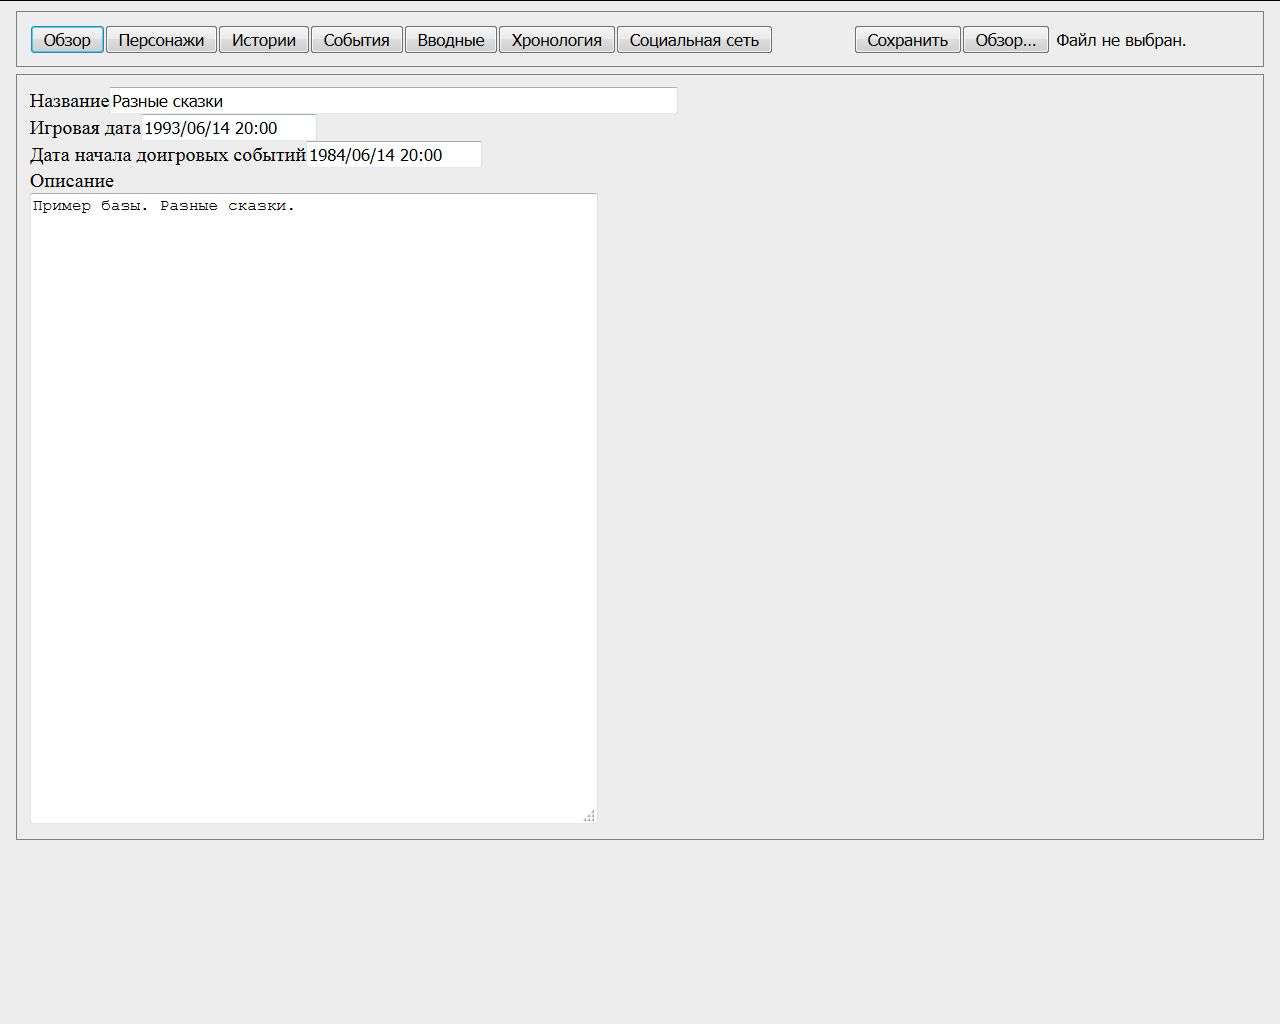
\includegraphics{1_overview.jpg}
\caption{Вкладка Обзор}\end{figure}
\newpage

\section{Персонажи}
\label{pages:id4}\label{pages:characters-desc}
На странице Персонажи есть общая часть и две дополнительных вкладки: досье и редактор досье.

Общая часть включает в себя элементы для создания/переименование/удаления персонажей в верхней части вкладки.
\begin{figure}[H]
\centering
\capstart

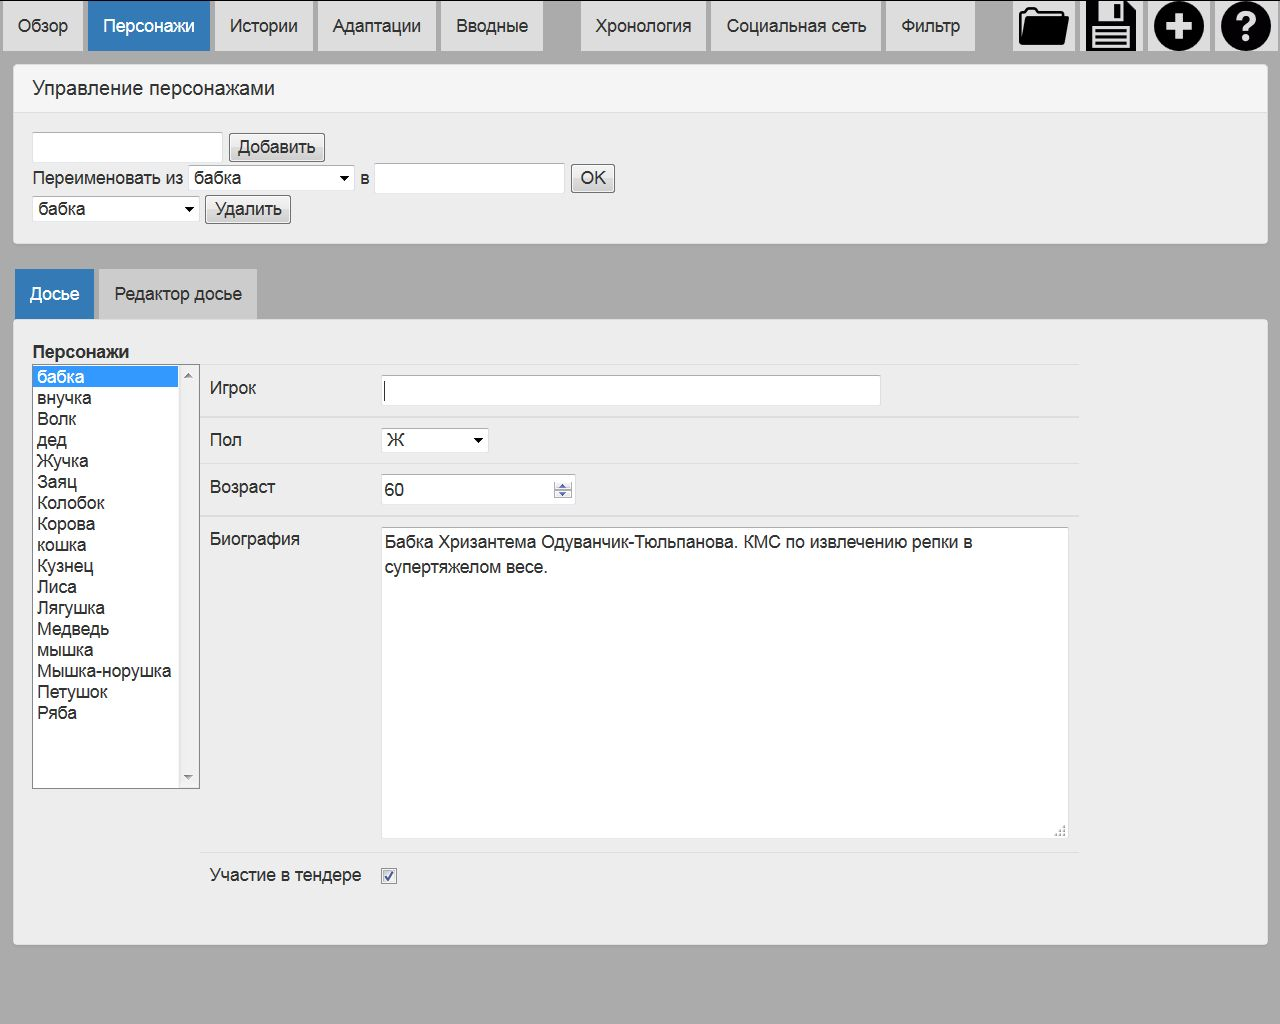
\includegraphics{2_1_characterProfile.jpg}
\caption{Вкладка Персонажи}\end{figure}
\newpage

\section{Персонажи. Досье}
\label{pages:id5}\label{pages:characters-profile}
На вкладке Досье происходит заполнение досье персонажа. В левой части экрана выбирается персонаж. По центру показано досье. Внесенные в досье изменения сохраняются автоматически. Подробнее про типы данных в досье можно прочитать в описании Редактора досье.
\begin{figure}[H]
\centering
\capstart

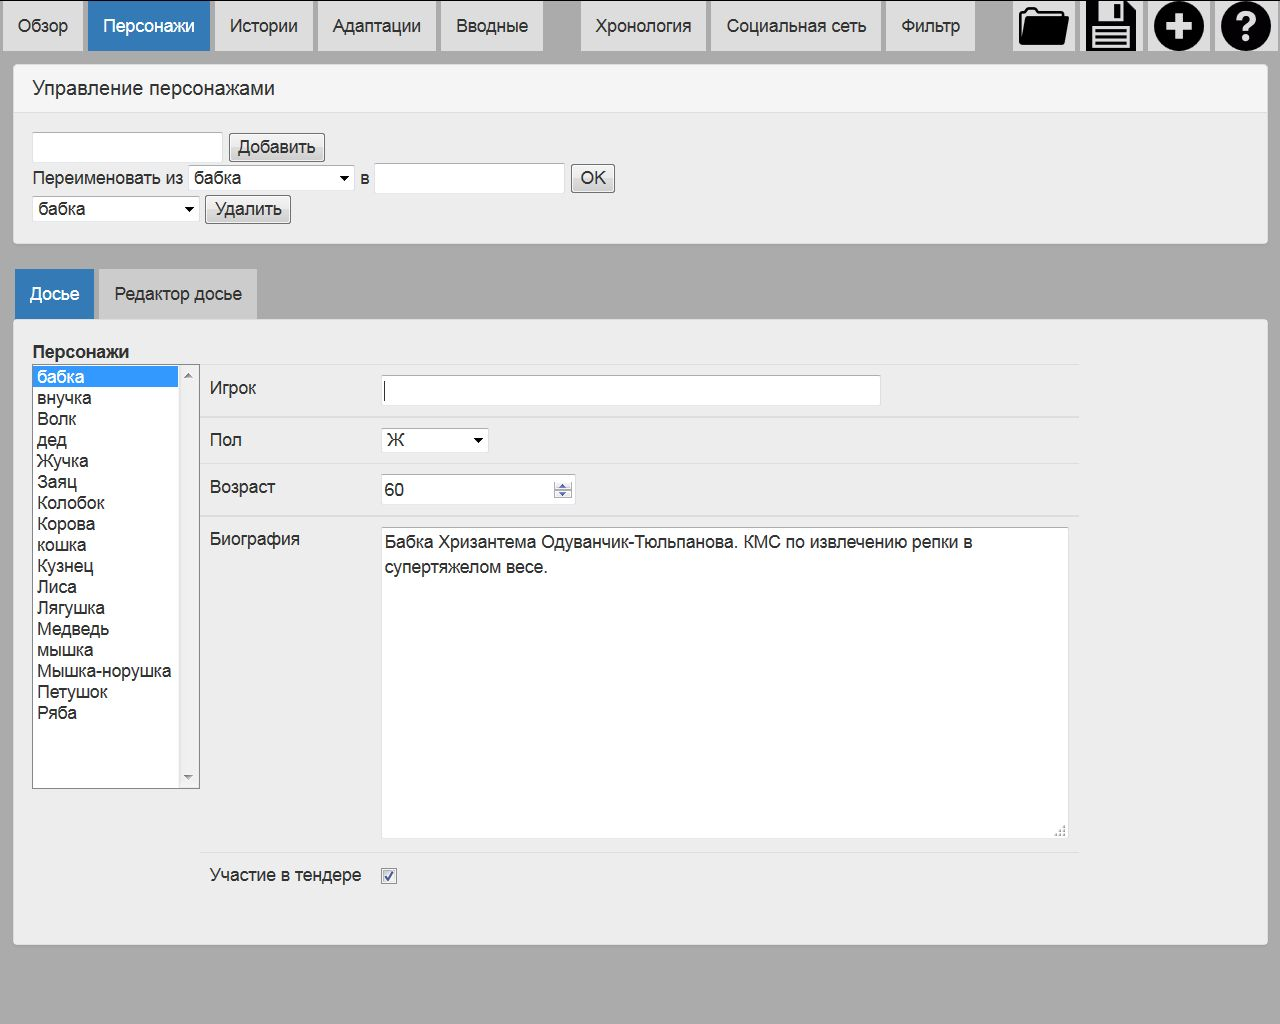
\includegraphics{2_1_characterProfile.jpg}
\caption{Вкладка Персонажи. Досье}\end{figure}
\newpage

\section{Персонажи. Редактор досье}
\label{pages:id6}\label{pages:characters-profile-editor}
На вкладке Редактор досье выполняется редактирование досье персонажей: добавление/изменение/удаление полей в досье. В верхней части вкладки находятся элементы управления для создания полей, перестановки полей и удаления полей. Имена полей должны быть уникальны. Все текущие поля показаны в таблице: название, тип и значения. То, что указано в поле \code{Значения} является значением по умолчанию для всех полей, кроме единственного выбора. В единственном выборе значением по умолчанию является первый элемент.

Типы полей:
\begin{quote}

\code{Текст} - поле для хранения текстовых данных. Пример: биография персонажа.

\code{Строка} - поле хранит одну строку. Пример: вероисповедание

\code{Единственный выбор} - поле содержащее перечисление значений из которых может быть выбрано только одно. Значения единственного выбора указываются через запятую. Первое значение является значением по умолчанию. Пример: пол ж, м, не важно

\code{Число} - числовое значение. Пример: возраст персонажа

\code{Галочка} - поле хранит значение да/нет.
\end{quote}
\begin{figure}[H]
\centering
\capstart

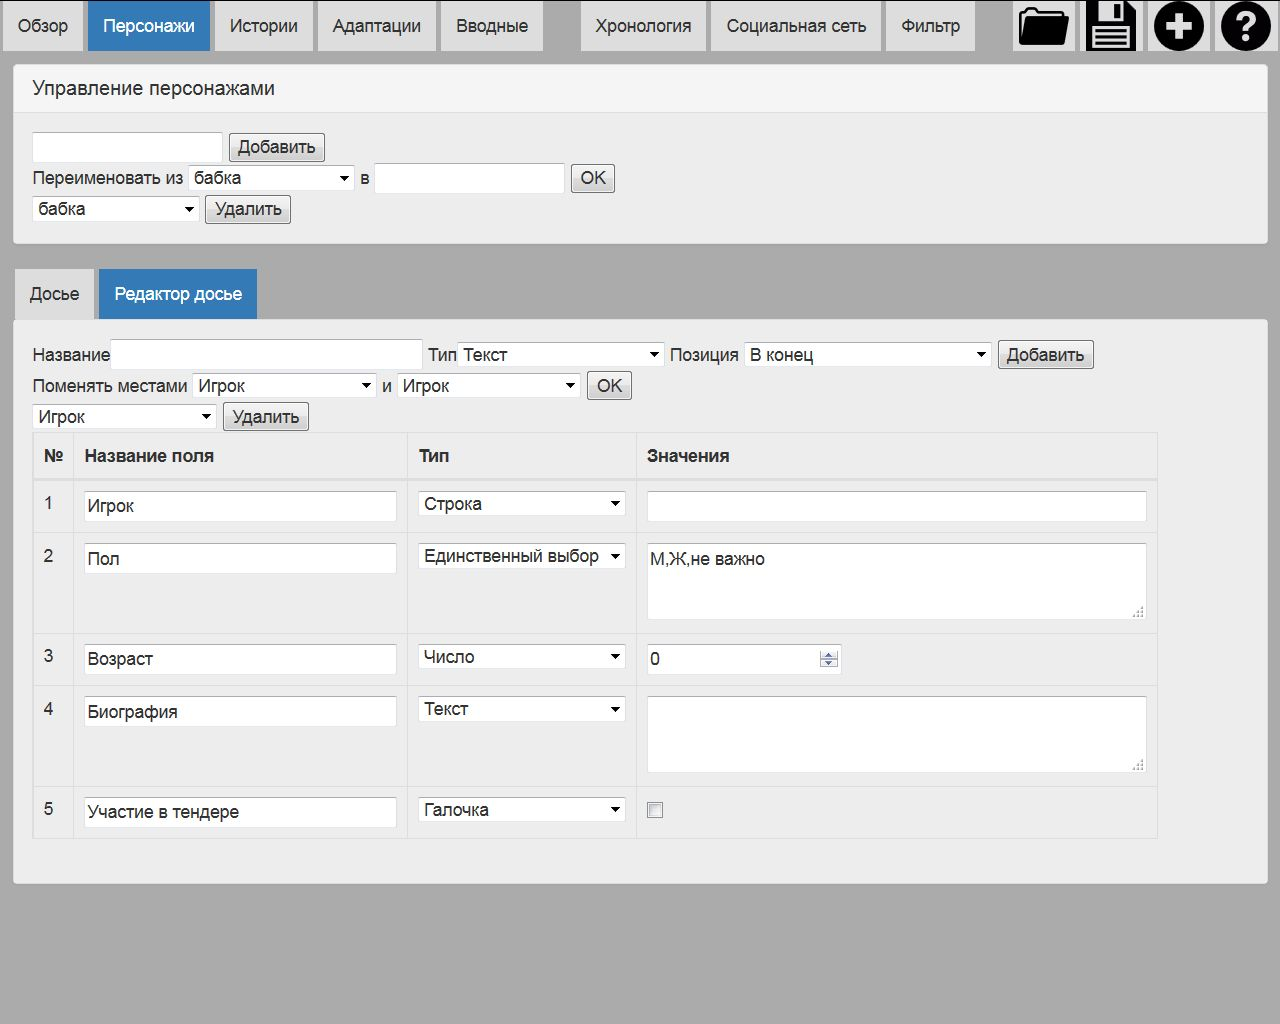
\includegraphics{2_3_characterPrfileConfigurer.jpg}
\caption{Вкладка Персонажи. Редактор досье}\end{figure}
\newpage

\section{Истории}
\label{pages:story-desc}\label{pages:id7}
На странице Истории осуществляется заполнение мастерских версий историй. В общую часть входят следующие элементы: создание/переименование/удаление историй, заполнение мастерской версии истории. Заполнять мастерскую версию не обязательно, но по нашему опыту бывает полезно иметь всю историю перед глазами. Поле для мастерской истории прячется/показывается при нажатии на кнопку \code{Мастерская история} для экономии места для других вкладок. Во всех последующих рисунках мастерская история спрятана.

В левой части экрана расположен элемент для выбора текущей истории.
\begin{figure}[H]
\centering
\capstart

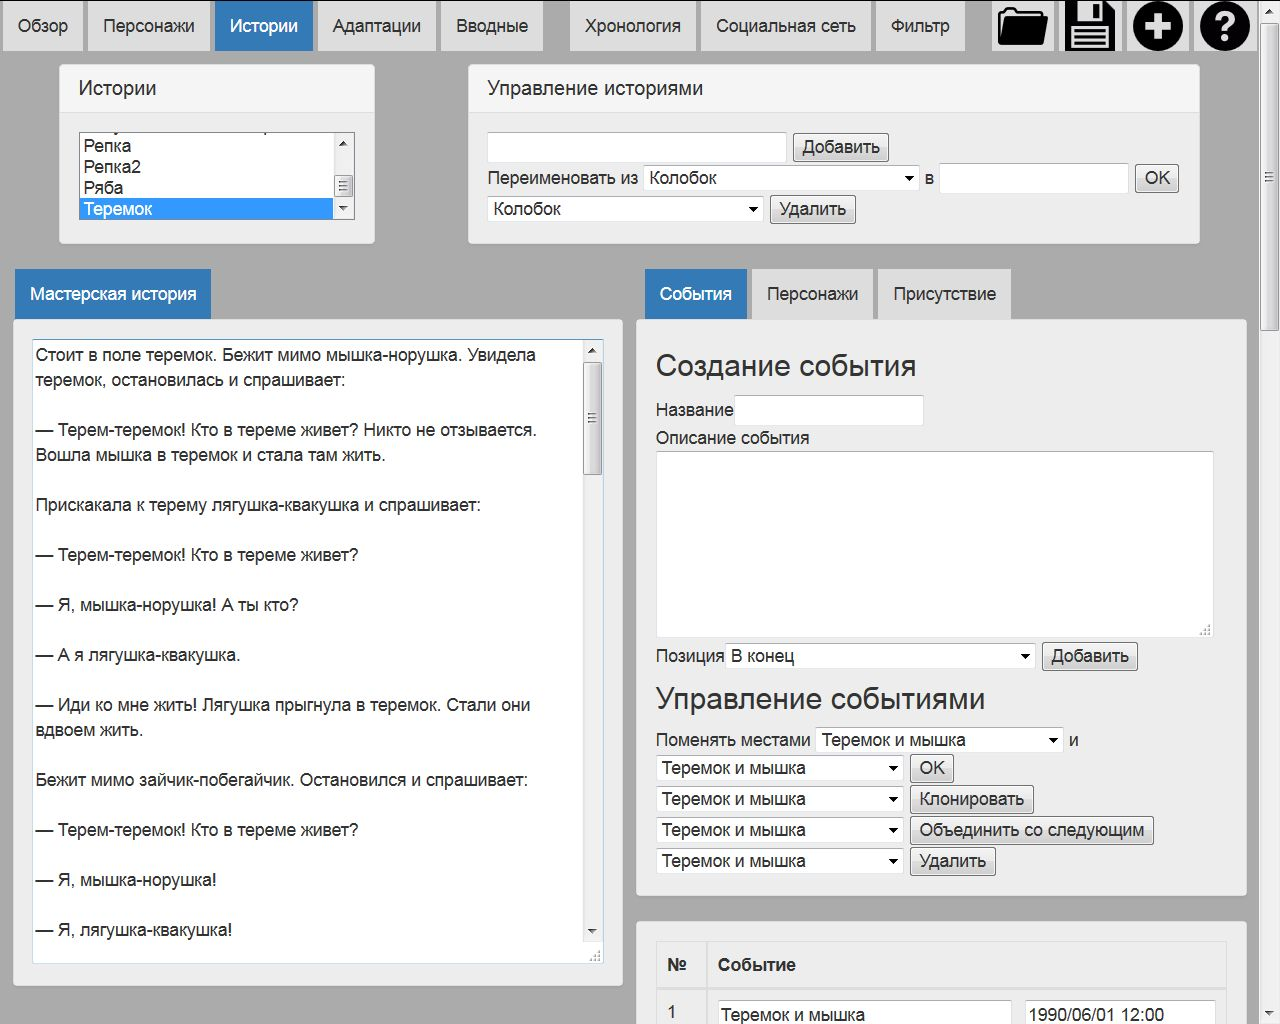
\includegraphics{3_0_masterStory.jpg}
\caption{Вкладка Истории}\end{figure}
\newpage

\section{Истории. События}
\label{pages:id8}\label{pages:story-events}
На вкладке события выполняется разбиение истории на события. У каждого события есть следующие атрибуты: название (не уникально), текст, позиция и время. Кроме обычных операций создания/удаления/перестановки событий добавлены операции клонирования и объединения событий. Клонирование создает полную копию события с созданием копии текстов адаптаций (см. раздел {\hyperref[pages:events-desc]{\emph{\DUspan{}{Адаптации}}}}). Объединение событий соединяет два подряд идущих события в одно. Объединяется все: название, описание и адаптации.

В таблице события приведены в том порядке, в котором их укажет мастер, а не в хронологическом порядке. Переименование и обновление текста событий сохраняется при завершении редактирования, то есть немедленно. Справа указано точное время наступления события. Если поле подсвечено красным, значит используется значение по умолчанию - время окончания доигровых событий.
\begin{figure}[H]
\centering
\capstart

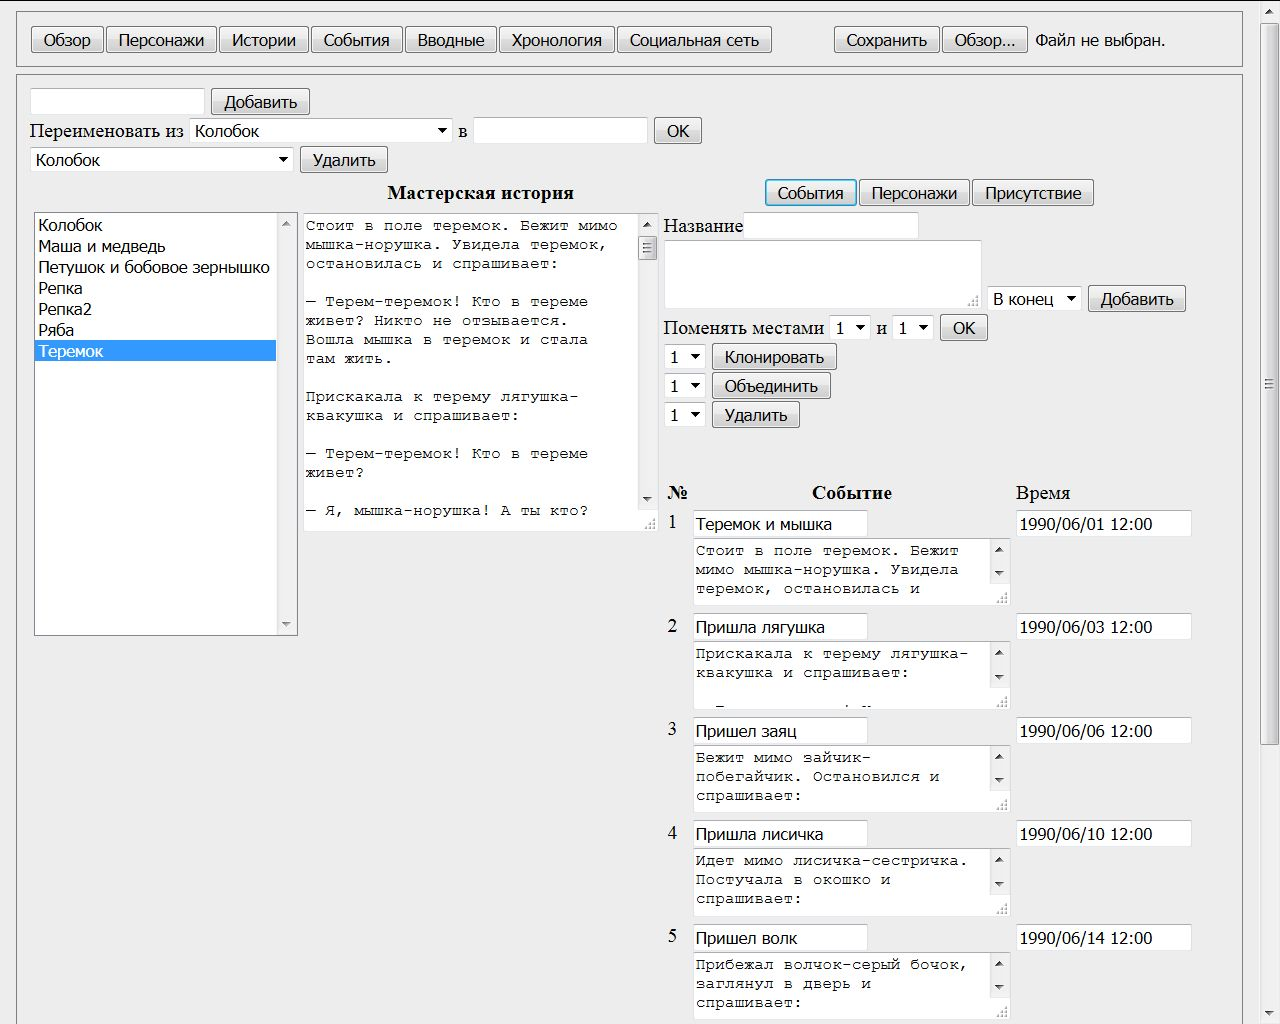
\includegraphics{3_1_storyEvents.jpg}
\caption{Вкладка События}\end{figure}
\newpage

\section{Истории. Персонажи}
\label{pages:story-characters}\label{pages:id9}
На вкладке Персонажи выполняется добавление/удаление/замещение персонажей в истории. При замещении все данные от старого персонажа переходят к новому. Так что да, Ромео не приехал, его место займет Меркуцио)

Здесь же приведено две таблицы. Первая таблица указывает вид активности персонажа в истории. Описание видов активности приведено в разделе {\hyperref[theory:secondary-entities-desc]{\emph{\DUspan{}{Вторичные сущности}}}}.
\begin{figure}[H]
\centering
\capstart

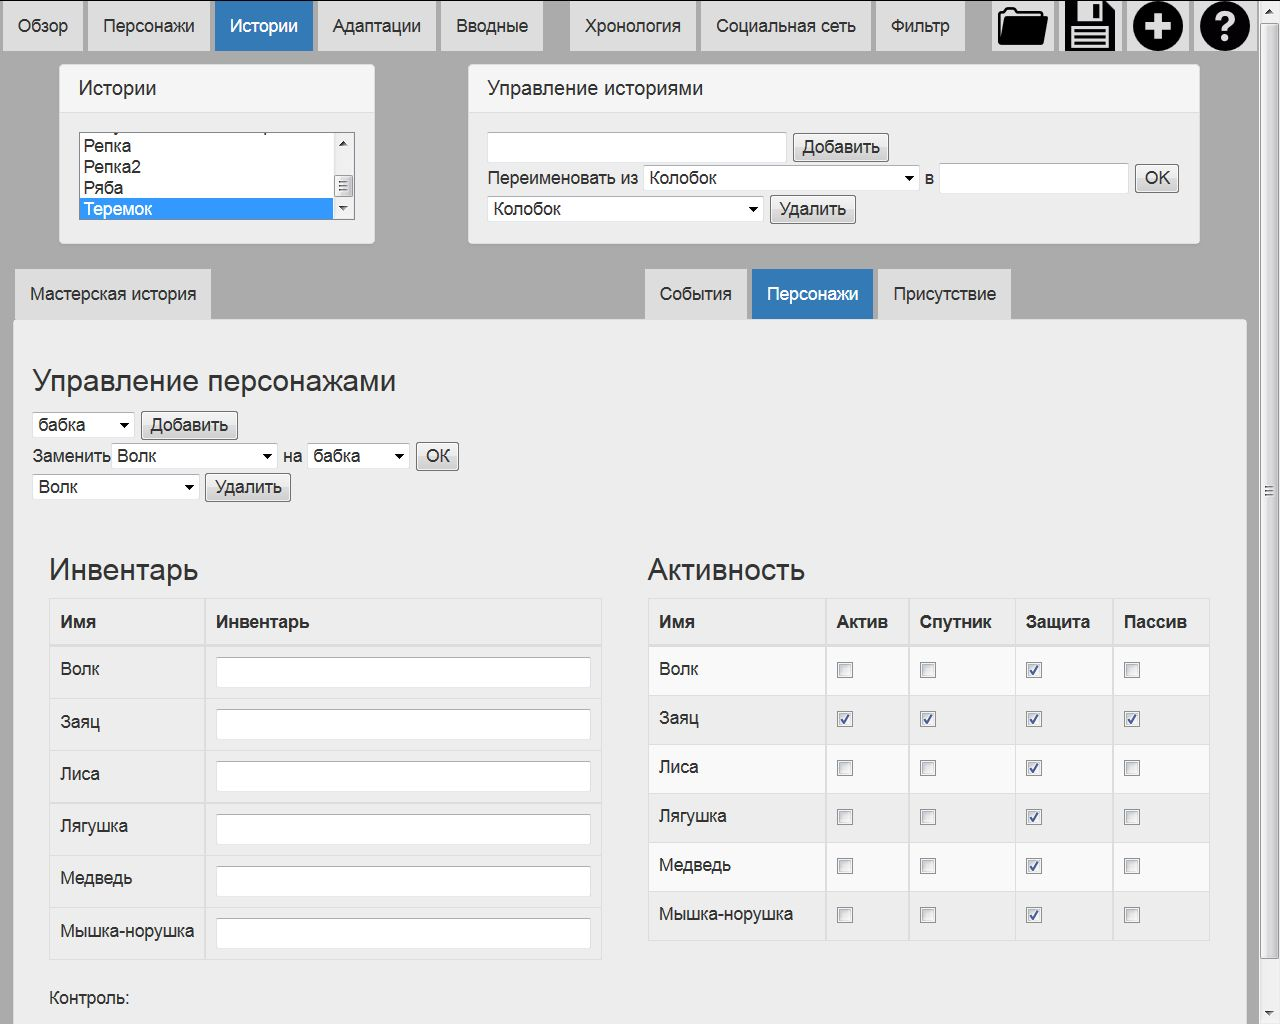
\includegraphics{3_2_storyCharacters.jpg}
\caption{Вкладка Истории. Персонажи}\end{figure}
\newpage

\section{Истории. Присутствие}
\label{pages:id10}\label{pages:story-presence}
На этой вкладке определяется участие персонажей в тех или иных событиях. В таблице в первом столбце перечислены названия событий. В заголовке имена персонажей истории. Отметьте галочками пересечение персонажа и события, если персонаж принял в них участие. Снятие галочки приводит к удалению уже существующих адаптаций событий (см. раздел {\hyperref[pages:events-desc]{\emph{\DUspan{}{Адаптации}}}}). На всякий случай в этом месте всегда выскакивает напоминалка.
\begin{figure}[H]
\centering
\capstart

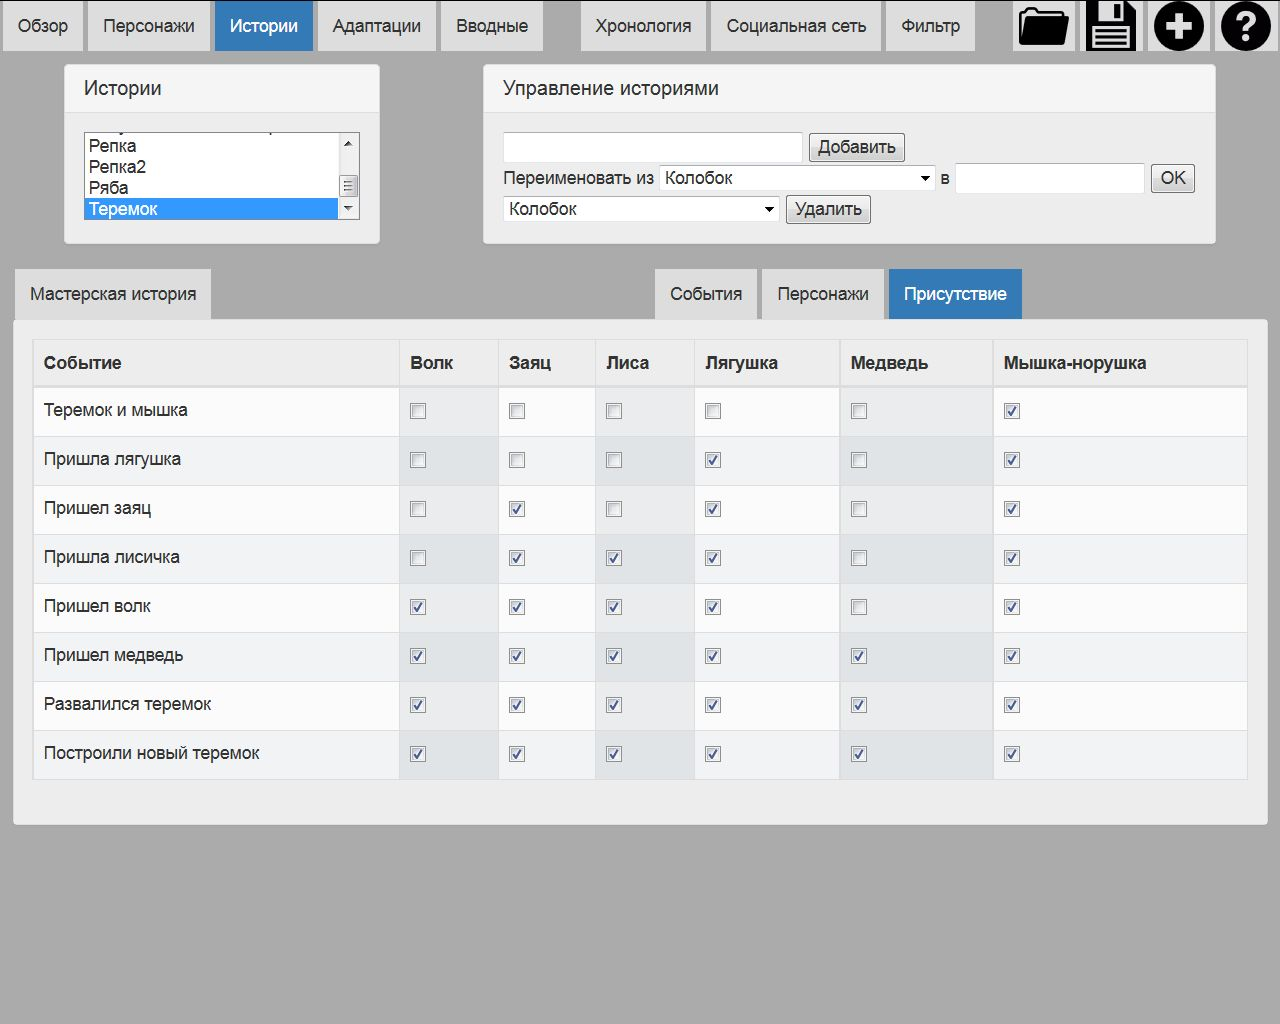
\includegraphics{3_3_eventPresence.jpg}
\caption{Вкладка Истории. Присутствие}\end{figure}
\newpage

\section{Адаптации}
\label{pages:id11}\label{pages:events-desc}
У каждого персонажа может быть свое видение происходящих событий, поэтому для событий необходимо сделать адаптацию как это событие выглядело с точки зрения того или иного персонажа.

Слева сверху расположен селектор истории (единственный выбор). Слева снизу расположен селектор персонажей (множественный выбор через ctrl). По центру отображаются таблица из двух столбцов. В левом столбце выводится оригинальное описание события, которое можно редактировать. В правом столбце выводятся текстовые поля с описанием события для каждого выбранного персонажа - текст адаптации. Таким образом в один момент времени можно работать, как с адаптацией одного персонажа, так и с несколькими персонажами одновременно. Под текстом адаптации выводится галочка - отметка о завершении работы над адаптацией. Сверху расположена галочка-фильтр завершенных историй. История считается завершенной, если проставлены галочки о завершении всех адаптаций.
\begin{figure}[H]
\centering
\capstart

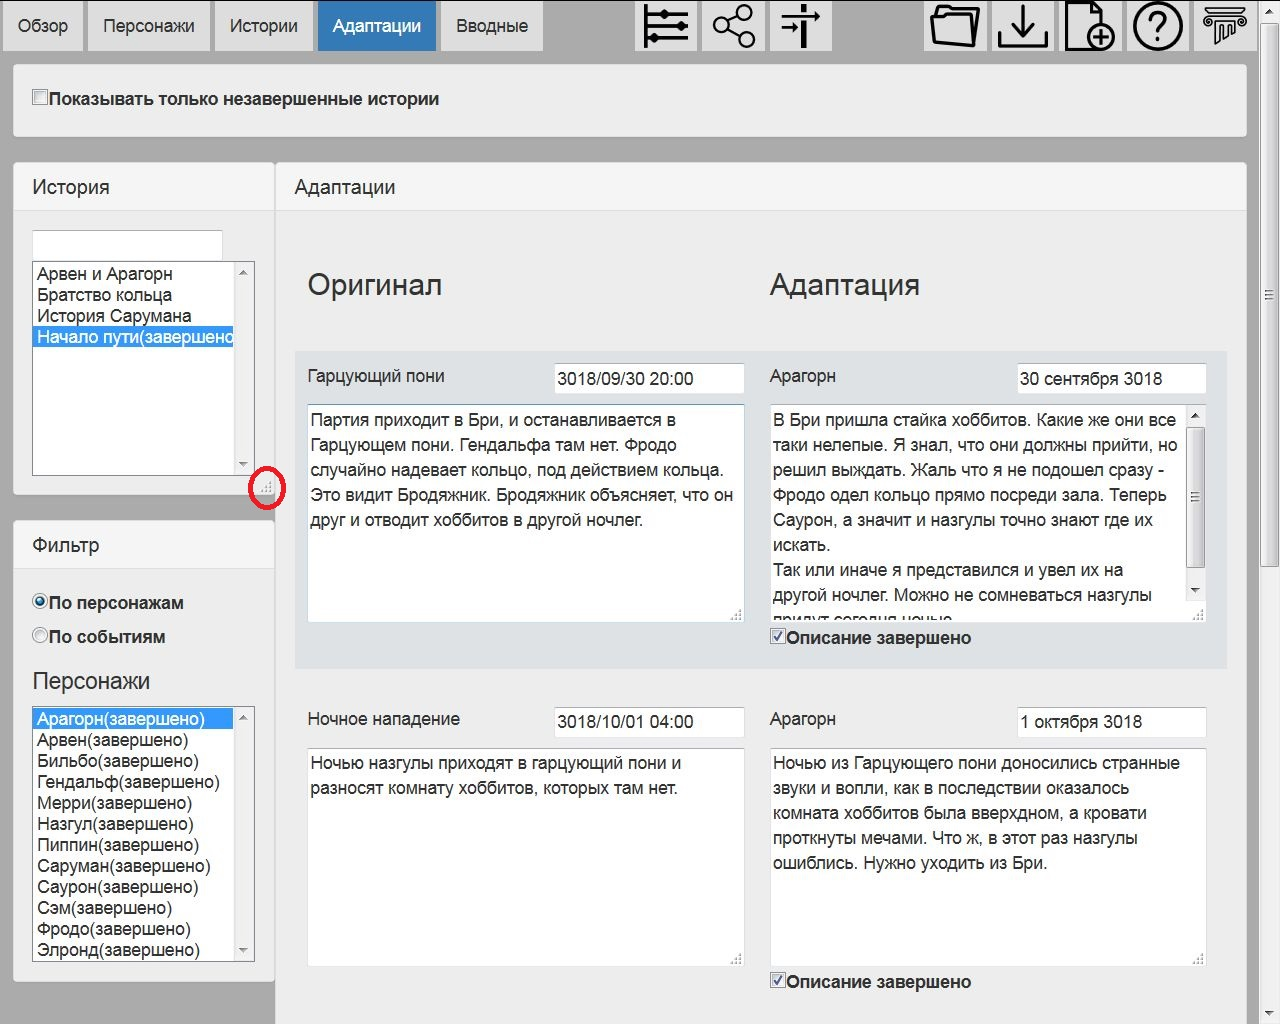
\includegraphics{4_events.jpg}
\caption{Вкладка События}\end{figure}
\newpage

\section{Вводные. Предварительный просмотр}
\label{pages:breifings-preview}\label{pages:id12}
Прежде чем экспортировать вводные, можно посмотреть какая информация будет выведена, используя вкладку предварительного просмотра. При предварительном просмотре необходимо указать тип отображения событий: в хронологическом порядке или сгруппированными по историям. Под этим выбором находится селектор персонажа. Инвентарь и адаптации событий можно редактировать из режима предварительного просмотра. Обращаю ваше внимание - в заголовке события указывается ключевое поле \code{История} или \code{Персонаж}. Если это \code{История}, значит для персонажа не была написана адаптация текста события и он увидит его как есть. Редактирование такого поля является редактированием текста события. Если в заголовке указано \code{Персонаж}, значит вы редактируете адаптацию события.
\begin{figure}[H]
\centering
\capstart

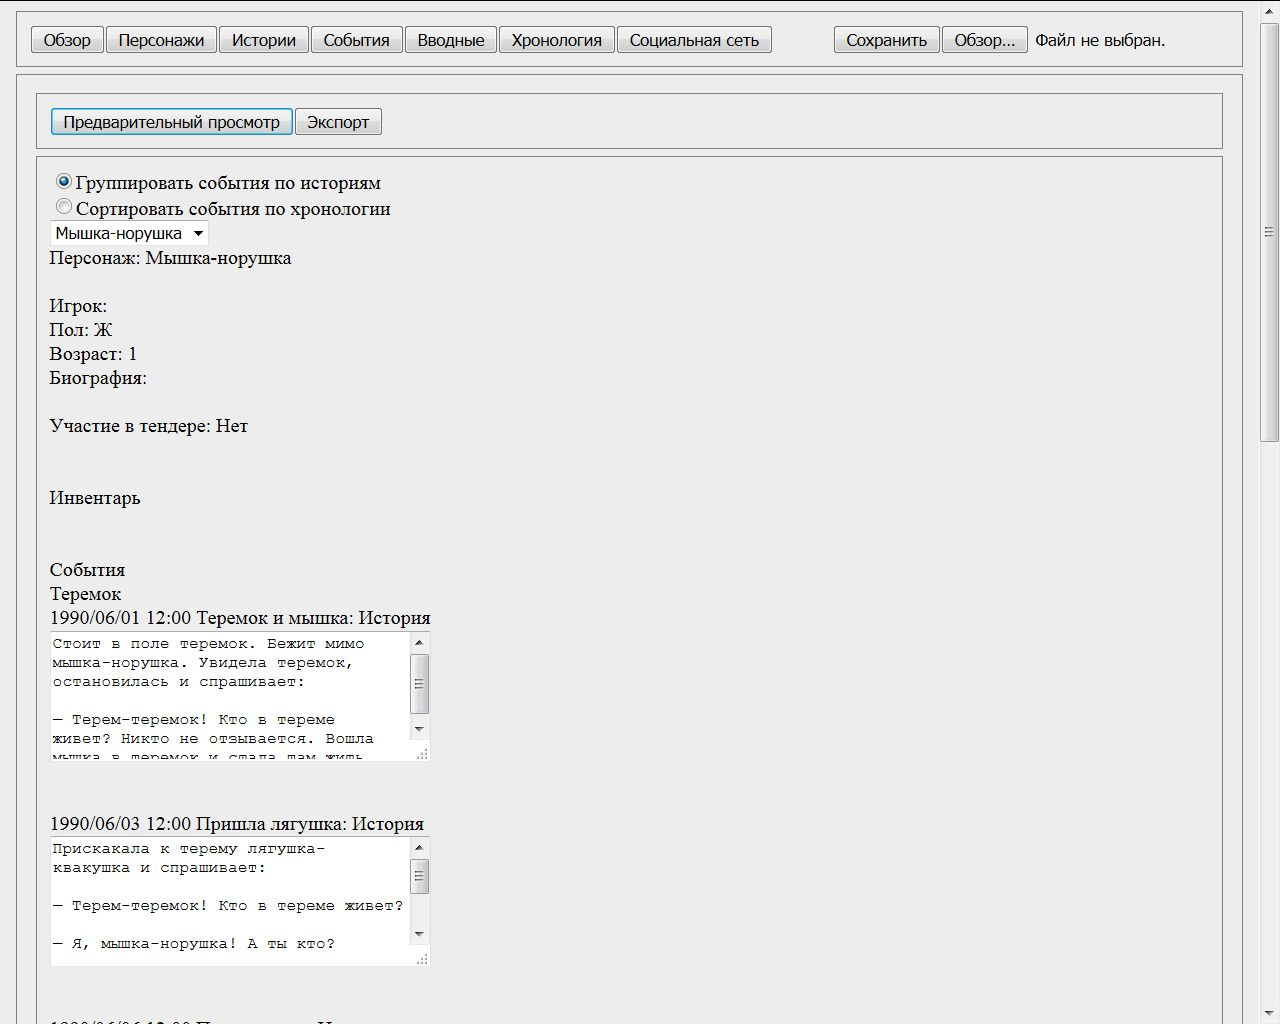
\includegraphics{5_1_briefingPreview.jpg}
\caption{Вкладка Вводные. Предварительный просмотр}\end{figure}
\newpage

\section{Вводные. Экспорт}
\label{pages:id13}\label{pages:breifings-export}
На вкладке экспорта доступны следующие опции. Вводные можно выводить одним файлом, либо каждую в отдельный файл. Во втором случае вводные будут выгружены в zip архиве. В разделе Простая выгрузка перечислены несколько встроенных шаблонов: \code{выгрузка в docx c событиями по хронологии}, \code{выгрузка в docx c событиями по историям}, \code{выгрузка таблицы с инвентарем} и \code{выгрузка в текстовый файл}.

В разделе продвинутой выгрузки необходимо указать тип используемого шаблона и загрузить свой собственный шаблон. Шаблон может включать в себя как все данные, так и только часть из них. Примеры шаблонов распространяются вместе с НИМС.
\begin{figure}[H]
\centering
\capstart

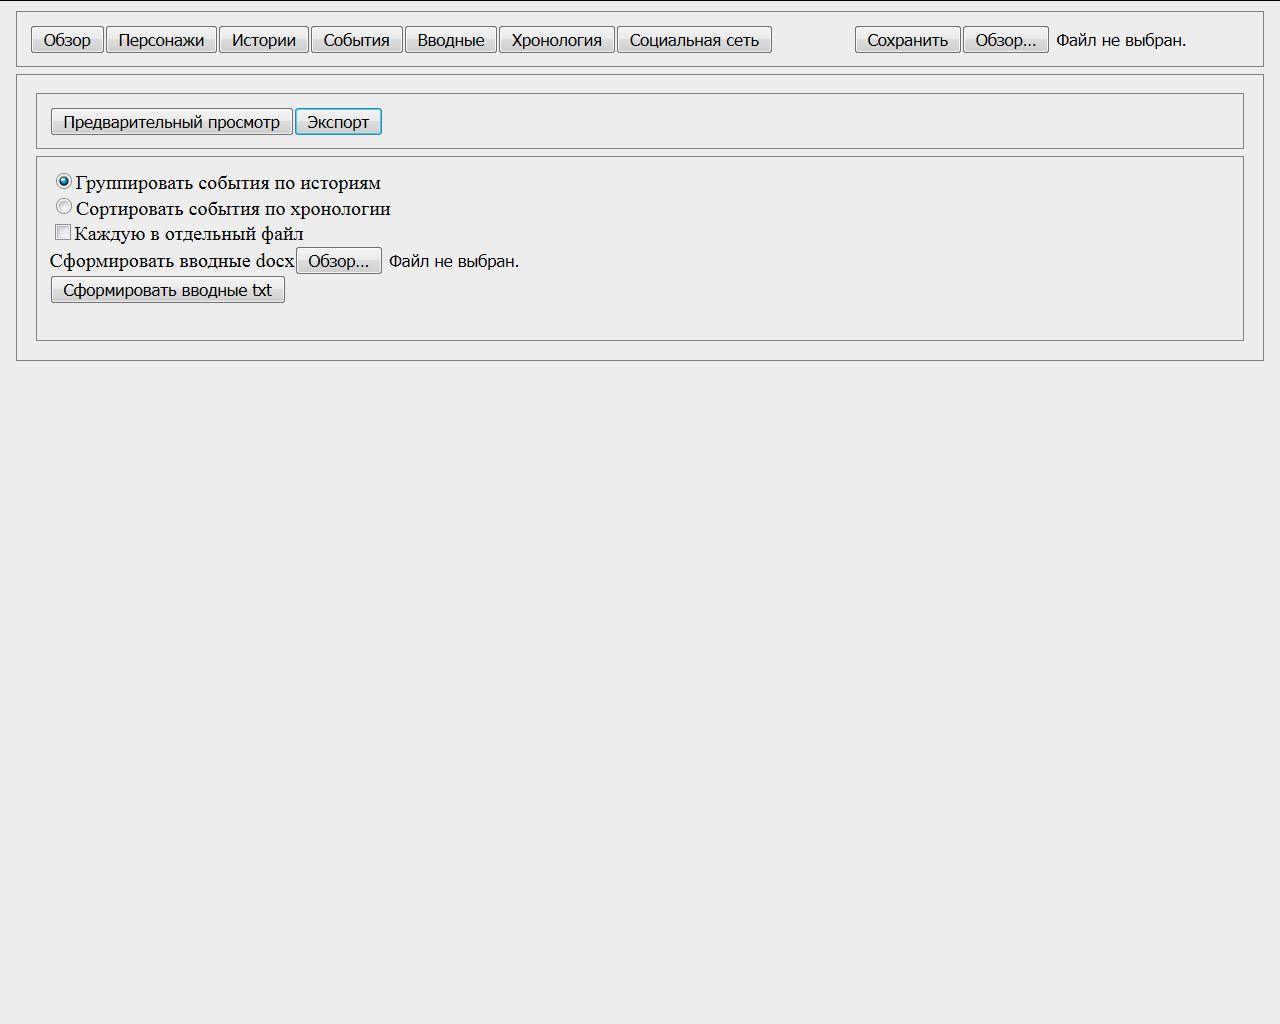
\includegraphics{5_2_briefingExport.jpg}
\caption{Вкладка Вводные. Экспорт}\end{figure}
\newpage

\section{Хронология}
\label{pages:id14}\label{pages:timeline-desc}
На этой вкладке отображается хронология событий. Слева находится селектор событий. Чтобы сделать множественный выбор зажмите ctrl и выбирайте элементы в списке. Масштаб хронологии изменяется с помощью колесика мыши. Красным отмечено время начала и завершения доигровых событий. События можно перетаскивать по хронологии. Для этого нажмите ЛКМ на событии и тащите его в нужную сторону. При этом следует учитывать, что от этих перемещений время событий в историях меняется автоматически.
\begin{figure}[H]
\centering
\capstart

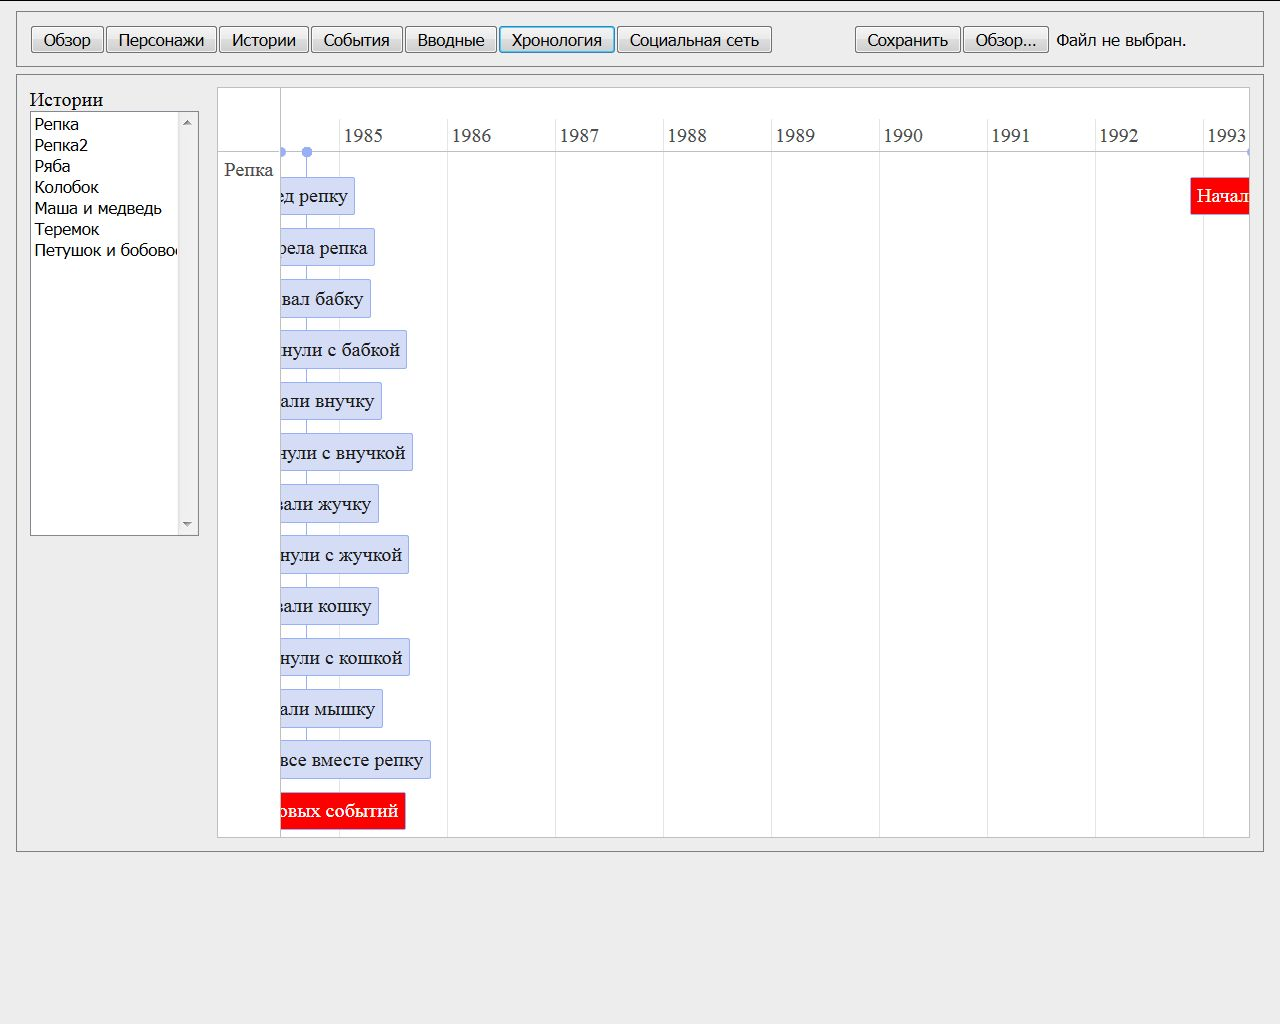
\includegraphics{6_timeline.jpg}
\caption{Вкладка Хронология}\end{figure}
\newpage

\section{Социальная сеть}
\label{pages:social-network-desc}\label{pages:id15}
На этой вкладке отрисовываются социальные сети на основе имеющихся данных. Поддерживаются несколько типов отрисовываемых сетей с разными видами узлов и связей между ними (см. далее типы графов). Отрисовка социальной сети требует большого количества ресурсов, поэтому перед ее использованием рекомендуется сохранить текущее состояние базы. Для отрисовки необходимо указать общие и частные параметры социальной сети и нажать кнопку \code{Нарисовать}.

Общие параметры

Раскраска узлов выполняется на основе полей досье c типом \textbf{единственный выбор} и \textbf{галочка}. Вы можете выбрать любое из этих полей, а ниже будет приведена цветовая расшифровка.
Так же возможно три вида выборки.
\begin{enumerate}
\item {}
Все данные. Будут отрисованы все данные.

\item {}
Избранные персонажи. В этом случае появится список персонажей. Можно выбрать нескольких персонажей с помощью ctrl. В этом случае будут отрисованы выбранные персонажи, все истории, в которых задействованы эти персонажи и все остальные персонажи, пересекающиеся в событиях с избранными. Примечание: при отрисовке графа человек-история не все связи отображают реальные связи персонажей по событиям.

\item {}
Избранные истории. В этом случае появится список историй. Можно выбрать несколько историй с помощью ctrl. В этом случае будут отрисованы все истории и все персонажи, входящие в истории.

\end{enumerate}

Частной настройкой является тип отрисовываемого графа. Поддерживаются следующие типы.
\begin{enumerate}
\item {}
Детальная сеть - сеть связей между персонажами. Узлы: персонажи. Связь между узлами: совместное участие персонажей в некотором событии. Чем толще связь, тем в больших историях эти персонажи пересекаются. При наведении на связь выводится список историй, в которых пересекаются эти персонажи.

\item {}
Человек-история - сеть связей персонажей и историй. Узлы: персонажи и истории. Связь между узлами: участие персонажа в истории. Размер истории пропорционален числу участников истории.

\item {}
Человек-история 2 - сеть связей персонажей и историй на основе данных об активности. Узлы: персонажи и истории. Связь между узлами: активность персонажа в истории. См. раздел с описанием активностей. Можно выбирать несколько требуемых активностей через ctrl.

\end{enumerate}
\begin{figure}[H]
\centering
\capstart

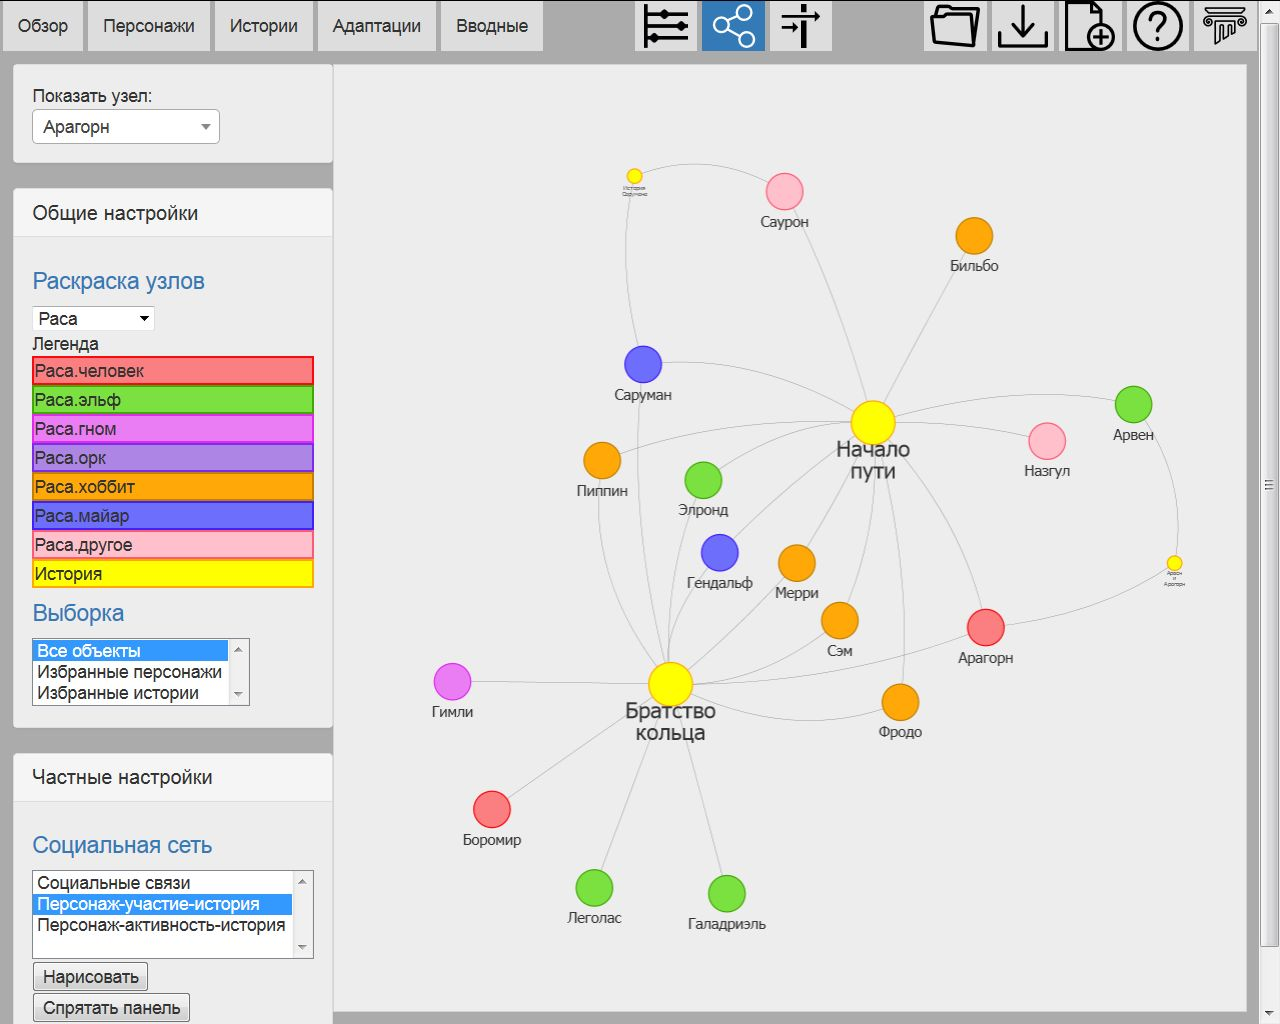
\includegraphics{7_socialNetwork.jpg}
\caption{Вкладка Социальная сеть}\end{figure}

\newpage

\section{Фильтр}
\label{pages:id16}\label{pages:characters-filter}
На вкладке Фильтр выполняется выборка из персонажей по досье. Подробнее про типы данных в досье можно прочитать в разделе {\hyperref[pages:characters-profile-editor]{\emph{\DUspan{}{Персонажи. Редактор досье}}}}. Фильтрация строк и текстов происходит по наличию искомой строки в строке или тексте. Фильтрация по полям с единственным выбором происходит по выбору из предложенного списка значений. Чтобы сделать множественный выбор зажмите ctrl и выбирайте элементы в списке. Фильтрация для значений вида да/нет аналогична фильтрации по полям с единственным выбором. Фильтрация по числовым значениям требует указания числа и вида проверки: не важно, больше, равно, меньше. Обновление результата фильтрации происходит сразу после изменения параметров фильтра. В центральной части выводится результат фильтрации. Клик по заголовку таблицы выполняет сортировку по соответствующему полю + иконка.
\begin{figure}[H]
\centering
\capstart

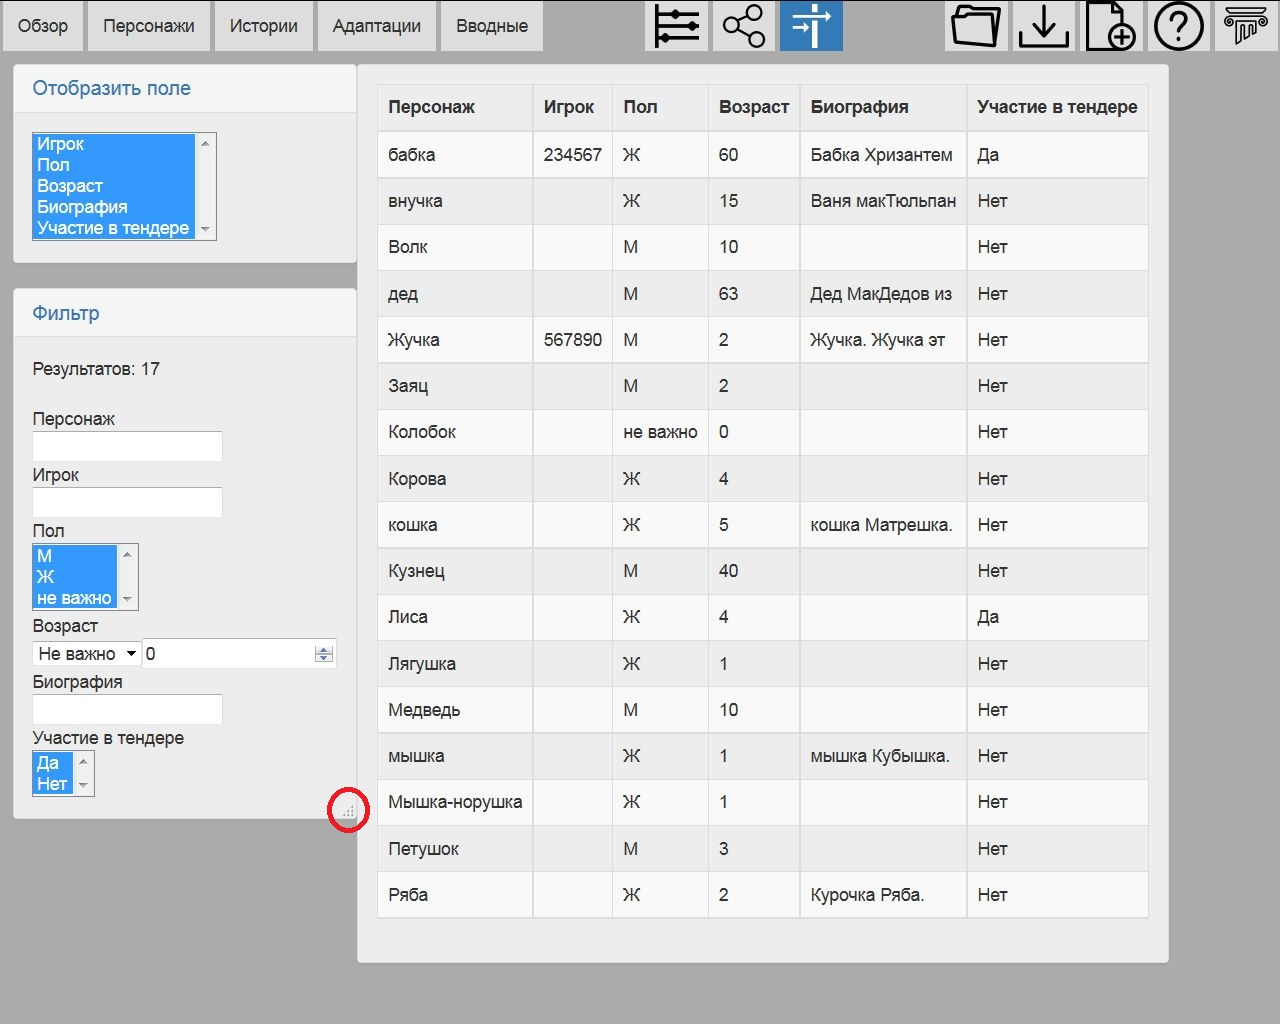
\includegraphics{2_2_characterFilter.jpg}
\caption{Вкладка Фильтр}\end{figure}



\renewcommand{\indexname}{Алфавитный указатель}
\printindex
\end{document}
